\section{Elements Formation and Distribution}

%\subsection{Angular Dependence}

\begin{frame}{Elements distribution's dependence on $\theta$}
\begin{columns}
\column{0.6\textwidth}
\vfill
\centering
% --- First row ---

\includegraphics[width=0.45\linewidth]{../fig/blh_vlr_hr_constatm/Masses_sections_theta.pdf}%
\hspace{0.04\linewidth}%

\includegraphics[width=0.45\linewidth]{../fig/sfho_vlr_hr_constatm/Masses_sections_theta.pdf}

\vspace{2mm} % vertical space between rows

% --- Second row ---

\includegraphics[width=0.45\linewidth]{../fig/dd2_135_vlr_hr_constatm/Masses_sections_theta.pdf}%
\hspace{0.04\linewidth}%

\includegraphics[width=0.45\linewidth]{../fig/dd2_180_vlr_hr_constatm/Masses_sections_theta.pdf}

\column{0.4\textwidth}

\begin{itemize}
\scriptsize
	\item Bulk of heavy elements for $\theta\lesssim36^{o}$
	\item Largest mass of heavy $r$-process elements on top of remnant for DD2\_q1.67
	\item SFHo\_q1.0 has the smaller production of H and He 

\end{itemize}
\end{columns}
\end{frame}

\begin{frame}{Elements distribution's dependence on $\phi$}
\begin{columns}
\column{0.6\textwidth}


\centering
% --- First row ---

\includegraphics[width=0.45\linewidth]{../fig/blh_vlr_hr_constatm/Masses_sections_phi.pdf}%
\hspace{0.04\linewidth}%

\includegraphics[width=0.45\linewidth]{../fig/sfho_vlr_hr_constatm/Masses_sections_phi.pdf}

\vspace{2mm} % vertical space between rows

% --- Second row ---

\includegraphics[width=0.45\linewidth]{../fig/dd2_135_vlr_hr_constatm/Masses_sections_phi.pdf}%
\hspace{0.04\linewidth}%

\includegraphics[width=0.45\linewidth]{../fig/dd2_180_vlr_hr_constatm/Masses_sections_phi.pdf}


\column{0.4\textwidth}

\begin{itemize}
\scriptsize
	\item SFHo\_q1.0 and DD2\_q1.0 have higher $\phi$-impact on elements as  $^{134}_{54}Xe$
	\item SFHo\_q1.0 and DD2\_q1.0 elements production not affected by a factors $\gtrsim2$ 
	\item Largest variation for BLh\_q1.43 and DD2\_q1.67 found for $A\gtrsim134$ 
	\item  BLh\_q1.43 and DD2\_q1.67 element production can be affected by factors of $\sim5-10$ 

\end{itemize}
\end{columns}
\end{frame}




\begin{frame}{Sky Maps}
    \begin{itemize}
        \item Sky 
        \item Maps
    \end{itemize}
\end{frame}

%\subsection{Time Dependence}

\begin{frame}{Temporal Dependence}
\begin{columns}
\column{0.6\textwidth}

\centering
% --- First row ---

\includegraphics[width=0.3\linewidth]{../fig/blh_vlr_hr_constatm/BLH_polar.pdf}%
\hspace{0.04\linewidth}%

\includegraphics[width=0.3\linewidth]{../fig/sfho_vlr_hr_constatm/SFHO_polar.pdf}

\vspace{2mm} % vertical space between rows

% --- Second row ---

\includegraphics[width=0.3\linewidth]{../fig/dd2_135_vlr_hr_constatm/DD2S_polar.pdf}%
\hspace{0.04\linewidth}%

\includegraphics[width=0.3\linewidth]{../fig/dd2_180_vlr_hr_constatm/DD2A_polar.pdf}

\end{figure}

\column{0.4\textwidth}

\begin{itemize}
\scriptsize
\item Feed WinNet with datasets evolved for 300ms and 1sec
\item Symmetric binaries are not highly affected
\item Polar regions of BLh\_q1.43 is mostly affected in the first $r$-process peak
\item Polar regions of DD2\_q1.67 is mostly affected for $A\gtrsim130$
\item Lanthanides and Actinides expansion (?)
\item 
\end{itemize}

\end{columns}
\end{frame}

\begin{frame}{Temporal Dependence}
\begin{figure}
    \centering
    
\includegraphics[width=0.9\linewidth]{../fig/dd2_180_vlr_hr_constatm/Sky_locations_compare.pdf}
\end{figure}


\end{frame}

%\subsection{$^{56}_{28}$Ni production}


\begin{frame}{$^{56}_{28}$Ni impact}

\begin{columns}[T] % T = topo alinhado


\column{0.7\textwidth}

\centering
% --- First row ---
\includegraphics[width=0.45\linewidth]{../fig/blh_vlr_hr_constatm/Energy_evolution_zoom_BLH_q1.43.pdf}%
\hspace{0.04\linewidth}%
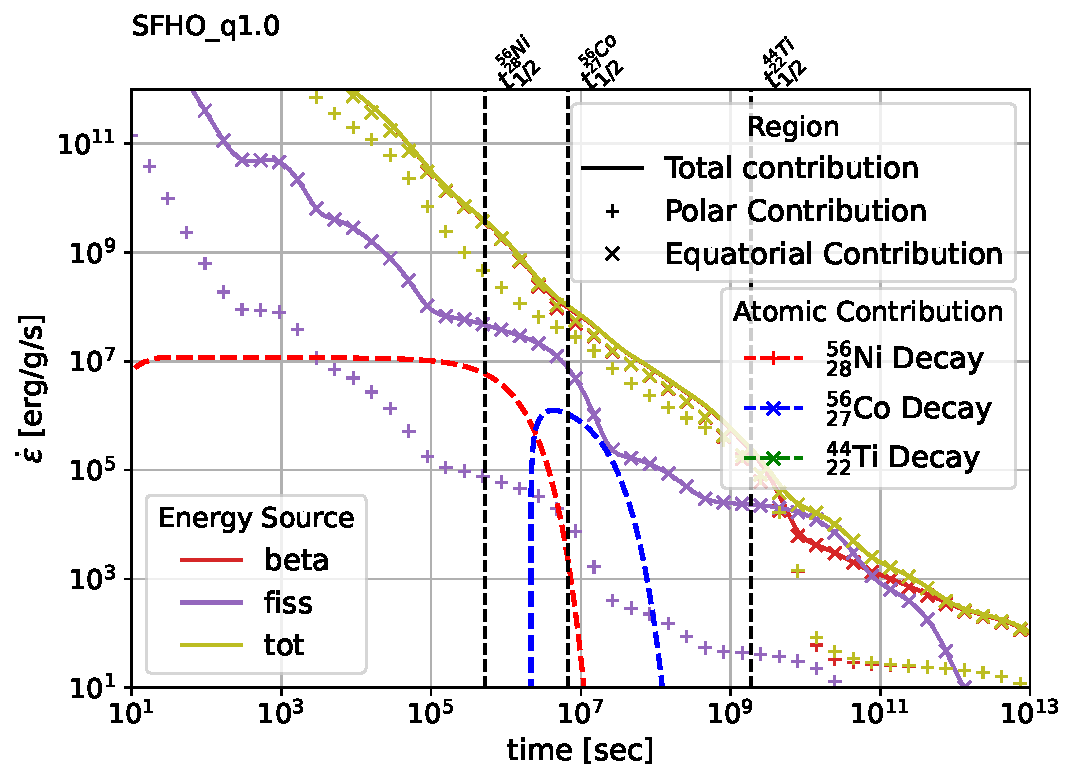
\includegraphics[width=0.45\linewidth]{../fig/sfho_vlr_hr_constatm/Energy_evolution_zoom_SFHO_q1.0.pdf}

\vspace{2mm} % vertical space between rows

% --- Second row ---

\includegraphics[width=0.45\linewidth]{../fig/dd2_135_vlr_hr_constatm/Energy_evolution_zoom_DD2_q1.0.pdf}%
\hspace{0.04\linewidth}%

\includegraphics[width=0.45\linewidth]{../fig/dd2_180_vlr_hr_constatm/Energy_evolution_zoom_DD2_q1.67.pdf}

\column{0.3\textwidth}

\begin{tcolorbox}[
    colback=white,
    colframe=blue,
    colbacktitle=blue!50!black!50,
    title=Ejecta masses,
    fonttitle=\bfseries,
    rounded corners,
    boxrule=1pt,
    left=2mm, right=2mm, top=1mm, bottom=1mm
]
\tiny
\setlength{\tabcolsep}{2pt}
\begin{tabular}{c|c}
\hline\hline
Model & $M_{\mathrm{ej}}[M_{\odot}]$ \\
\hline\hline
BLh\_q1.43 & $8.37\times10^{-3}$ \\
\hline
SFHo\_q1.0 & $4.58\times10^{-3}$ \\
\hline
DD2\_q1.0  & $4.63\times10^{-3}$ \\
\hline
DD2\_q1.67 & $1.38\times10^{-2}$ \\
\hline\hline
\end{tabular}
\end{tcolorbox}

\vspace{2mm}

\begin{tcolorbox}[
    colback=white,
    colframe=blue,
    colbacktitle=blue!50!black!50,
    title=Nickel masses,
    fonttitle=\bfseries,
    rounded corners,
    boxrule=1pt,
    left=2mm, right=2mm, top=1mm, bottom=1mm
]
\tiny
\setlength{\tabcolsep}{2pt}
\begin{tabular}{c|c}
\hline\hline
Model & $M_{\mathrm{ej}}^{^{56}_{28}\mathrm{Ni}}[M_{\odot}]$ \\
\hline\hline
BLh\_q1.43 & $4.60\times10^{-4}$ \\
\hline
SFHo\_q1.0 & $1.10\times10^{-6}$ \\
\hline
DD2\_q1.0  & $1.59\times10^{-4}$ \\
\hline
DD2\_q1.67 & $3.10\times10^{-4}$ \\
\hline\hline
\end{tabular}
\end{tcolorbox}

\end{columns}
\end{frame}

